\documentclass[a4paper,12pt]{article}
\usepackage{xeCJK}          % 中文支持
\usepackage{fontspec}       % 英文/数学字体
\usepackage{amsmath, amssymb} % 数学公式
\usepackage{graphicx}       % 插入图片
\usepackage{hyperref}       % 目录超链接
\usepackage{geometry}       % 页面布局
\usepackage{bm}             % 粗体
\usepackage{xcolor}         % 颜色
\usepackage{tabularx}       % 表格环境
\usepackage{tikz}           % TikZ 绘制主对角线斜线
\usepackage{tcolorbox}
\usepackage{xstring}
\usepackage{pgfplots}
\usepackage{enumitem}
\usepackage{pifont}
\usepackage{ulem}
\usepackage{mathtools}
\usepackage{dsfont}
\usepackage{extarrows}
\pgfplotsset{compat=1.18}
\geometry{left=3cm,right=3cm,top=3cm,bottom=3cm}

\definecolor{customgreen}{rgb}{0.2,0.6,0.3}
\newcommand{\gmath}[1]{\textcolor{customgreen}{#1}}

% 经典
\definecolor{classicgreen}{rgb}{0.1,0.5,0.3}
\newtcbox{\classic}{
    on line,
    colback=classicgreen!10,
    colframe=classicgreen,
    boxrule=0.8pt,
    arc=3pt,
    boxsep=1pt,
    left=4pt,
    right=4pt,
    top=2pt,
    bottom=2pt
}


\definecolor{customgreen}{rgb}{0.2,0.6,0.3}

% 抽离颜色和尺寸参数
\newcommand{\analysisTitleColor}{green!50!black}
\newcommand{\analysisBackColor}{white}
\newcommand{\analysisBoxRule}{0.8pt}
\newcommand{\analysisArc}{3pt}
\newcommand{\analysisPadding}{6pt}

% 定义 tcolorbox
\newtcolorbox{analysisbox}[1][]{
    title=\IfStrEq{#1}{}{\textbf{解析}}{#1}, % 如果传参为空则使用“解析”
    colback=\analysisBackColor,
    colframe=\analysisTitleColor,
    boxrule=\analysisBoxRule,
    arc=\analysisArc,
    left=\analysisPadding,
    right=\analysisPadding,
    top=4pt,
    bottom=4pt
}

\newlist{circlenum}{enumerate}{1}
\setlist[circlenum]{
    label=\ding{\numexpr171+\arabic*},
    leftmargin=2.2em,
    itemsep=0.6em,      % item 之间的距离（主要）
    topsep=0.6em,       % 列表与上下正文的距离
    parsep=0.3em,       % item 内段落的间距
    partopsep=0.3em     % 列表前后额外间距
}

\newcommand{\blueuline}[1]{{\color{blue}\uline{\color{black}{#1}}}}

% =========================
% 字体设置
% =========================
\setmainfont{Times New Roman}
\setsansfont{Helvetica Neue}
\setmonofont{Menlo}
\setCJKmainfont{PingFang SC}

% =========================
% 图形路径（可调整）
% =========================
\graphicspath{{./assets/}}

% =========================
% 文档开始
% =========================
\begin{document}

%    \title{Template}
%    \author{Bowen}
%    \date{\today}
%    \maketitle
%    \tableofcontents
%    \newpage


% =========================

    \section{多元函数微分学}

    \subsection{基本概念}

    \subsubsection{邻域}

    设 $P_0(x_0, y_0)$ 是 $xOy$ 平面上的一个点，$\delta$ 是某一正数。

    \begin{enumerate}
        \item \textbf{$\delta$ 邻域}：与点 $P_0(x_0, y_0)$ 距离小于 $\delta$ 的点 $P(x,y)$ 的全体，称为点 $P_0$ 的 $\delta$ 邻域，记为 $U(P_0, \delta)$：
        \[
            U(P_0, \delta) = \left\{ (x,y) \mid \sqrt{(x-x_0)^2 + (y-y_0)^2} < \delta \right\}
        \]

        \item \textbf{$\delta$ 去心邻域}：点 $P_0$ 的去心 $\delta$ 邻域记为 $\mathring{U}(P_0, \delta)$：
        \[
            \mathring{U}(P_0, \delta) = \left\{ (x,y) \mid 0 < \sqrt{(x-x_0)^2 + (y-y_0)^2} < \delta \right\}
        \]

        \item \textbf{$\delta$ 邻域的几何意义}：$U(P_0, \delta)$ 表示$xOy$ 平面上以点 $P_0(x_0, y_0)$ 为中心，$\delta > 0$ 为半径的圆内部的点 $P(x,y)$ 的全体
    \end{enumerate}

    \subsubsection{极限}

    \begin{enumerate}
        \item \textbf{定义}：设函数 $f(x,y)$ 在区域$D$上有定义，$P_0(x_0, y_0) \in D$或为区域$D$边界上一点。如果对于任意给定的 $\varepsilon > 0$，总存在 $\delta > 0$，使得当点 $P(x,y) \in D$，且满足$0 < |PP_0| = \sqrt {(x-x_0)^2 + (y-y_0)^2} < \delta$ 时，恒有
        \[
            |f(x,y) - A| < \varepsilon
        \]
        则称常数 $A$ 为函数 $f(x,y)$ 当 $(x,y) \to (x_0,y_0)$ 时的极限，记为
        \[
            \lim_{(x,y) \to (x_0,y_0)} f(x,y) = A \quad \text{或} \quad \lim_{\substack{x \to x_0 \\ y \to y_0}} f(x,y) = A
        \]

        \item \textbf{说明}
        \begin{itemize}
            \item 二重极限存在，要求 $P(x,y)$ 以\textbf{任意方式}（任意路径）趋于 $P_0(x_0,y_0)$ 时，$f(x,y)$ 都无限接近于 $A$
            \item \textbf{极限不存在的证明方法}：
            \begin{circlenum}
                \item 找两条不同路径，使极限值不同
                \item 某一路径使极限不存在
            \end{circlenum}
            \item 除洛必达法则和单调有界准则外，二重极限保持了一元极限的唯一性、局部有界性、局部保号性、运算规则、脱帽法和夹逼准则
        \end{itemize}

        \item \textbf{常用极限}：
        \begin{itemize}
            \item $\displaystyle\lim_{(x,y) \to (0,0)} \frac{x^2y}{x^2+y^2} = 0$（有界量 $\times$ 无穷小）
            \item $\displaystyle\lim_{(x,y) \to (0,0)} \frac{xy}{\sqrt{x^2+y^2}} = 0$
        \end{itemize}

    \end{enumerate}

    \subsubsection{连续}

    \begin{enumerate}
        \item \textbf{定义}：如果$\lim\limits_{(x,y) \to (x_0,y_0)} f(x,y) = f(x_0, y_0)$，则称函数 $f(x,y)$ 在点 $P_0(x_0,y_0)$ 处\textbf{连续}，如果$f(x, y)$在区域$D$上每一点处都连续，则称$f(x, y)$在区域$D$上\textbf{连续}
        \item \textbf{连续函数的性质}：在有界闭区域 $D$ 上连续的二元函数具有以下性质
        \begin{circlenum}
            \item \textbf{有界性定理}：在 $D$ 上必有界
            \item \textbf{最值定理}：在 $D$ 上必能取得最大值和最小值
            \item \textbf{介值定理}：必能取得介于最大值和最小值之间的任何值
        \end{circlenum}
    \end{enumerate}

    \subsubsection{偏导数}

    \begin{enumerate}
        \item \textbf{定义}：设函数 $z = f(x,y)$ 在点 $(x_0, y_0)$ 的某一邻域内有定义，如果极限
        \[
            \lim_{\Delta x \to 0} \frac{f(x_0 + \Delta x, y_0) - f(x_0, y_0)}{\Delta x}
        \]
        存在，则称此极限为函数 $z = f(x,y)$ 在点 $(x_0,y_0)$ 处对 $x$ 的\textbf{偏导数}，记为
        \[
            \frac{\partial z}{\partial x}\bigg|_{\substack{x=x_0 \\ y=y_0}}, \quad \frac{\partial f}{\partial x}\bigg|_{\substack{x=x_0 \\ y=y_0}}, \quad z'_x\big|_{\substack{x=x_0 \\ y=y_0}}, \quad f'_x(x_0, y_0),  \quad \frac{\partial f(x_0, y_0)}{\partial x}
        \]
        即
        \[
            f'_x(x_0, y_0) = \lim_{\Delta x \to 0} \frac{f(x_0 + \Delta x, y_0) - f(x_0, y_0)}{\Delta x}
        \]
        类似地，函数 $z = f(x,y)$ 在点 $(x_0,y_0)$ 处对 $y$ 的\textbf{偏导数}定义为
        \[
            f'_y(x_0, y_0) = \lim_{\Delta y \to 0} \frac{f(x_0, y_0 + \Delta y) - f(x_0, y_0)}{\Delta y}
        \]
        \item 如果$z = f(x, y)$在区域$D$上的每一点$(x , y)$处都有偏导数，一般来说，它们仍是$x, y$的函数，则称为$f(x, y)$的偏导函数，简称偏导数，记作
        \[
            \frac{\partial z}{\partial x}, \quad \frac{\partial f}{\partial x}, \quad f'_x(x, y), \quad \frac{\partial z}{\partial y}, \quad \frac{\partial f}{\partial y}, \quad f'_y(x, y)
        \]

        \item \textbf{几何意义}：设有二元函数 $z = f(x, y)$，且$z_0 = f(x_0, y_0)$，则
        \begin{itemize}
            \item $f'_x(x_0, y_0)$ 在几何上表示曲线 $\begin{cases}
                                                         z = f(x,y) \\ y = y_0
            \end{cases}$ 在点 $(x_0, y_0, z_0)$ 处的切线对 $x$ 轴的斜率
            \item $f'_y(x_0, y_0)$ 在几何上表示曲线 $\begin{cases}
                                                         z = f(x,y) \\ x = x_0
            \end{cases}$ 在点 $(x_0, y_0, z_0)$ 处的切线对 $y$ 轴的斜率
        \end{itemize}

        \item \textbf{高阶偏导数}：如果二元函数$z = f(x, y)$的偏导数$f'_x(x, y)$和$f'_y(x, y)$仍然具有偏导数，则它们的偏导数称为$z = f(x, y)$的二阶偏导数。
        \begin{itemize}
            \item $\displaystyle\frac{\partial}{\partial x}\left(\frac{\partial z}{\partial x}\right) = \frac{\partial^2 z}{\partial x^2} = f'_{xx}(x,y)$
            \item $\displaystyle\frac{\partial}{\partial y}\left(\frac{\partial z}{\partial x}\right) = \frac{\partial^2 z}{\partial x \partial y} = f'_{xy}(x,y)$
            \item $\displaystyle\frac{\partial}{\partial x}\left(\frac{\partial z}{\partial y}\right) = \frac{\partial^2 z}{\partial y \partial x} = f'_{yx}(x,y)$
            \item $\displaystyle\frac{\partial}{\partial y}\left(\frac{\partial z}{\partial y}\right) = \frac{\partial^2 z}{\partial y^2} = f'_{yy}(x,y)$
        \end{itemize}

        \item \textbf{混合偏导数相等的充分条件}：如果 $z = f(x,y)$ 的两个二阶混合偏导数 $\dfrac{\partial^2 z}{\partial x \partial y}$ 和 $\dfrac{\partial^2 z}{\partial y \partial x}$ 在区域 $D$ 内{\blueuline{连续}}，那么在该区域内这两个二阶混合偏导数必相等。即二阶混合偏导数在连续的条件下与求导的次序无关
    \end{enumerate}

    \subsubsection{可微}

    \begin{enumerate}
        \item \textbf{定义}：设函数 $z = f(x,y)$ 在点 $(x, y)$ 的某邻域内有定义，如果函数在 $(x, y)$ 的全增量
        \[
            \Delta z = f(x + \Delta x, y + \Delta y) - f(x, y)
        \]
        可表示为
        \[
            \Delta z = A\Delta x + B\Delta y + o(\rho)
        \]
        其中 $A$、$B$ 不依赖于 $\Delta x$、$\Delta y$ 而仅与点 $(x, y)$ 有关，$\rho = \sqrt{(\Delta x)^2 + (\Delta y)^2}$，且当$\Delta x \to 0, \Delta y \to 0$时，$o(\rho)$ 为 $\rho$ 的高阶无穷小，则称函数 $z = f(x,y)$ 在点 $(x, y)$ \textbf{可微}，而 $A\Delta x + B\Delta y$ 称为函数 $z = f(x,y)$ 在点 $(x, y)$ 的\textbf{全微分}，记为 $\mathrm{d}z$，即
        \[
            \mathrm{d}z = A\Delta x + B\Delta y = A\mathrm{d}x + B\mathrm{d}y
        \]

        \item \textbf{可微的必要条件}：若函数 $z = f(x,y)$ 在点 $(x,y)$ 可微分，则该函数在点 $(x,y)$ 的偏导数 $\dfrac{\partial z}{\partial x}$、$\dfrac{\partial z}{\partial y}$ 必定存在，且
        \[
            \mathrm{d}z = \frac{\partial z}{\partial x}\mathrm{d}x + \frac{\partial z}{\partial y}\mathrm{d}y
        \]

        $\color{red}{\bigstar}$注意：偏导数存在是可微的必要条件（\textbf{可微 $\Rightarrow$ 可偏导}），但\textbf{不是充分条件}。偏导数存在不一定可微。

        \textbf{与一元函数的对比}：一元函数可微 $\Leftrightarrow$ 可导，而多元函数可微 $\Rightarrow$ 可偏导（单向推出，不可逆）。

        \textbf{一元函数的等价性证明}：设 $y = f(x)$
        \begin{itemize}
            \item 可微 $\Rightarrow$ 可导：若 $f$ 在 $x$ 处可微，则 $\Delta y = A\Delta x + o(\Delta x)$，于是 $\displaystyle\lim_{\Delta x \to 0} \frac{\Delta y}{\Delta x} = A$，即 $f'(x) = A$ 存在
            \item 可导 $\Rightarrow$ 可微：若 $f'(x)$ 存在，即$\displaystyle\lim_{\Delta x \to 0} \frac{\Delta y}{\Delta x} = A \Rightarrow \frac{\Delta y}{\Delta x} = A + \alpha \Rightarrow \Delta y = A\Delta x + o(\Delta x) $，故 $f$ 在 $x$ 处可微
        \end{itemize}

        \textbf{多元函数不可逆的原因}：偏导数只反映沿坐标轴方向的变化率，不能保证沿任意方向都能用线性函数近似。

        \item \textbf{可微的充分条件}：若函数 $z = f(x,y)$ 在点 $(x, y)$ 的偏导数 $\dfrac{\partial z}{\partial x}$、$\dfrac{\partial z}{\partial y}$ 存在且{\blueuline{连续}}，则函数在点 $(x, y)$ 处可微
        \begin{enumerate}
            \item 在区域$D$上，若$d[f(x, y)] = 0(df = \dfrac{\partial z}{\partial x}\mathrm{d}x + \dfrac{\partial z}{\partial y}\mathrm{d}y)$或$\dfrac{\partial z}{\partial x} = \dfrac{\partial z}{\partial y} = 0$，则$f(x, y) \equiv C(\text{常数}), (x, y) \in D$
            \item 判别函数$z = f(x, y)$在点$(x_0, y_0)$处的偏导数是否连续，步骤如下
            \begin{circlenum}
                \item 用定义法求 $f'_x(x_0, y_0)$ 和 $f'_y(x_0, y_0)$
                \item 用公式法求 $f'_x(x, y)$ 和 $f'_y(x, y)$
                \item 检验 $\displaystyle\lim_{(x,y) \to (x_0, y_0)} f'_x(x, y) = f'_x(x_0, y_0)$ 和 $\displaystyle\lim_{(x,y) \to (x_0, y_0)} f'_y(x, y) = f'_y(x_0, y_0)$ 是否成立。若成立，则$z = f(x, y)$在点 $(x_0, y_0)$ 处的偏导数是连续的
            \end{circlenum}
            \item 
\includegraphics[width=\linewidth]{math/advanced-mathematics/pic13-6.png}
        \end{enumerate}

        \item \textbf{可微的判别步骤}：
        \begin{circlenum}
            \item 写出全增量$\Delta z = f(x_0 + \Delta x, y_0 + \Delta y) - f(x_0, y_0)$
            \item 写出线性增量$A\Delta x + B\Delta y$，其中$A = f'_x(x_0, y_0), B = f'_y(x_0, y_0)$
            \item 做极限
            \[
                \lim_{\substack{\Delta x \to 0 \\ \Delta y \to 0}} \frac{\Delta z - [A\Delta x + B\Delta y]}{\sqrt{(\Delta x)^2 + (\Delta y)^2}}
            \]
            若该极限等于$0$，则$z = f(x, y)$在点$(x_0, y_0)$处可微，否则，就不可微
        \end{circlenum}
    \end{enumerate}

    \subsection{多元函数微分法则}

    \subsubsection{链式求导规则}

    \begin{enumerate}
        \item \textbf{全导数}：$z = f(u,v)$，而 $u = \varphi(t)$，$v = \psi(t)$，则
        \begin{center}
            \begin{minipage}{0.5\textwidth}
                \[
                    \frac{\mathrm{d}z}{\mathrm{d}t} = \frac{\partial f}{\partial u}\frac{\mathrm{d}u}{\mathrm{d}t} + \frac{\partial f}{\partial v}\frac{\mathrm{d}v}{\mathrm{d}t}
                \]
            \end{minipage}%
            \begin{minipage}{0.4\textwidth}
                \centering
                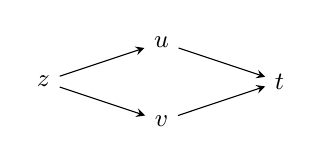
\begin{tikzpicture}
                    [every node/.style={font=\small}, >=stealth]
                    \node (z) at (0,0) {$z$};
                    \node (u) at (1.5,0.5) {$u$};
                    \node (v) at (1.5,-0.5) {$v$};
                    \node (t) at (3,0) {$t$};
                    \draw[->] (z) -- (u);
                    \draw[->] (z) -- (v);
                    \draw[->] (u) -- (t);
                    \draw[->] (v) -- (t);
                \end{tikzpicture}
            \end{minipage}
        \end{center}

        \item \textbf{偏导数}：$z = f(u,v)$，而 $u = \varphi(x,y)$，$v = \psi(x,y)$，则
        \begin{center}
            \begin{minipage}{0.5\textwidth}
                \[
                    \frac{\partial z}{\partial x} = \frac{\partial f}{\partial u}\frac{\partial u}{\partial x} + \frac{\partial f}{\partial v}\frac{\partial v}{\partial x}
                \]
                \[
                    \frac{\partial z}{\partial y} = \frac{\partial f}{\partial u}\frac{\partial u}{\partial y} + \frac{\partial f}{\partial v}\frac{\partial v}{\partial y}
                \]
            \end{minipage}%
            \begin{minipage}{0.4\textwidth}
                \centering
                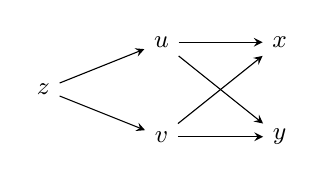
\begin{tikzpicture}
                    [every node/.style={font=\small}, >=stealth]
                    \node (z) at (0,0) {$z$};
                    \node (u) at (1.5,0.6) {$u$};
                    \node (v) at (1.5,-0.6) {$v$};
                    \node (x) at (3,0.6) {$x$};
                    \node (y) at (3,-0.6) {$y$};
                    \draw[->] (z) -- (u);
                    \draw[->] (z) -- (v);
                    \draw[->] (u) -- (x);
                    \draw[->] (u) -- (y);
                    \draw[->] (v) -- (x);
                    \draw[->] (v) -- (y);
                \end{tikzpicture}
            \end{minipage}
        \end{center}

        \item 全导数与偏导数的区别
        \begin{circlenum}
            \item \textbf{全导数} $\dfrac{\mathrm{d}z}{\mathrm{d}t}$：最终变量只有一个 $t$
            \item \textbf{偏导数} $\dfrac{\partial z}{\partial x}$：最终变量有多个（$x$, $y$）
        \end{circlenum}
    \end{enumerate}

    \textbf{记忆方法}：画出变量之间的依赖关系树形图，从 $z$ 到最终变量的每条路径上的偏导数相乘，所有路径的结果相加。

    \subsubsection{全微分形式不变性}

    设 $z = f(u,v)$ 具有连续偏导数，无论 $u$、$v$ 是自变量还是中间变量，都有
    \[
        \mathrm{d}z = \frac{\partial z}{\partial u}\mathrm{d}u + \frac{\partial z}{\partial v}\mathrm{d}v
    \]

    \textbf{应用}：求偏导数时，可以先求全微分，再比较系数。这种方法可以避免复杂的链式求导，减少出错。

    \begin{analysisbox}[Example]
        设 $z = u^2 v$，其中 $u = xy$，$v = x + y$，求 $\dfrac{\partial z}{\partial x}$ 和 $\dfrac{\partial z}{\partial y}$。

        \textbf{解}：利用全微分形式不变性
        \begin{align*}
            \mathrm{d}z &= \frac{\partial z}{\partial u}\mathrm{d}u + \frac{\partial z}{\partial v}\mathrm{d}v = 2uv\,\mathrm{d}u + u^2\,\mathrm{d}v \\
            &= 2uv(y\mathrm{d}x + x\mathrm{d}y) + u^2(\mathrm{d}x + \mathrm{d}y) \\
            &= (2uvy + u^2)\mathrm{d}x + (2uvx + u^2)\mathrm{d}y
        \end{align*}
        比较 $\mathrm{d}z = \dfrac{\partial z}{\partial x}\mathrm{d}x + \dfrac{\partial z}{\partial y}\mathrm{d}y$ 的系数，得
        \[
            \frac{\partial z}{\partial x} = 2uvy + u^2, \quad \frac{\partial z}{\partial y} = 2uvx + u^2
        \]
    \end{analysisbox}

    \subsubsection{隐函数存在定理（公式法）}

    \begin{enumerate}
        \item \textbf{隐函数存在定理1}（一个方程，两个变量）：对于由方程$F(x, y) = 0$确定的隐函数$y = f(x)$，当$F_y(x_0, y_0) \neq 0$时，则有
        \[
            \frac{\mathrm{d}y}{\mathrm{d}x} = {\color{red}{-}}\frac{F'_x(x, y)}{F'_y(x, y)}
        \]

        \item \textbf{隐函数存在定理2}（一个方程，三个变量）：对于由方程$F(x, y, z) = 0$确定的隐函数$z = f(x, y)$，当$F_z(x_0, y_0, z_0) \neq 0$时，则有
        \[
            \frac{\partial z}{\partial x} = {\color{red}{-}}\frac{F'_x(x, y, z)}{F'_z(x, y, z)}, \quad \frac{\partial z}{\partial y} = {\color{red}{-}}\frac{F'_y(x, y, z)}{F'_z(x, y, z)}
        \]
        \item \textbf{隐函数存在定理}：设 $F(x,y)$ 在点 $(x_0, y_0)$ 的某一邻域内具有连续的偏导数，且 $F(x_0, y_0) = 0$，则 $F'_y(x_0, y_0) \neq 0$ 是方程 $F(x, y) = 0$ 在点 $(x_0, y_0)$ 的某一邻域内能确定一个连续函数 $y = y(x)$，且满足 $y_0 = y(x_0)$，并有连续导数的\textbf{充分非必要条件}。
    \end{enumerate}

    \subsubsection{二元函数的拉格朗日定理}

    设$f(x, y)$定义在区域$D$上，且$\dfrac{\partial [f(x, y)]}{\partial x} = 0, \dfrac{\partial [f(x, y)]}{\partial y} = 0, (x, y) \in D$，则$f(x, y) = C(\text{常数}), (x, y) \in D$

    \subsection{多元函数的极值与最值}

    \subsubsection{概念}

    \begin{enumerate}
        \item 若存在点$(x_0, y_0)$的某个邻域，使得在该邻域内任意一点$(x, y)$处，均有
        \[
            f(x, y) \leq f(x_0, y_0)(\text{或}f(x, y) \geq f(x_0, y_0))
        \]
        成立，则称点$(x_0, y_0)$为$f(x, y)$的极大值点（或极小值点），$f(x_0, y_0)$为$f(x, y)$的\textbf{极大值}（或\textbf{极小值}）

        \item 设$(x_0, y_0)$为$f(x, y)${\blueuline{定义域}}在内一点，若对于$f(x, y)$的定义域内任意一点$(x, y)$，均有
        \[
            f(x, y) \leq f(x_0, y_0)(\text{或}f(x, y) \geq f(x_0, y_0))
        \]
        成立，则称$f(x_0, y_0)$为$f(x, y)$在$D$上的\textbf{最大值}（或\textbf{最小值}）

        \item 极值与最值的区别
        \begin{circlenum}
            \item \textbf{极值}：局部概念，只在某邻域内比较
            \item \textbf{最值}：全局概念，在整个区域$D$上比较
            \item \textbf{关系}：最值点$\subseteq$极值点$\cup$边界点
        \end{circlenum}
        \item 驻点、极值点的关系
        \begin{circlenum}
            \item \textbf{驻点}：使 $f'_x = 0$ 且 $f'_y = 0$ 的点
            \item \textbf{极值点}：局部最大或最小的点
            \item \textbf{重要}：极值点 $\subseteq$ 驻点（可微情形）；驻点不一定是极值点。
        \end{circlenum}

    \end{enumerate}

    \subsubsection{无条件极值}

    \begin{enumerate}
        \item \textbf{二元函数取极值的必要条件}：设函数 $z = f(x,y)$ 在点 $(x_0, y_0)$ 处 \begin{cases}
                                                                                             \text{一阶偏导数存在} \\
                                                                                             \text{有极值}
        \end{cases} 则有
        \[
            f'_x(x_0, y_0) = 0, \quad f'_y(x_0, y_0) = 0
        \]
        \begin{itemize}
            \item 该必要条件同样适用于三元即三元以上函数
            \item 偏导数不存在的点也可能是极值点
            \item 找可疑点\begin{cases}
                              f'_x(x_0, y_0) = 0, \quad f'_y(x_0, y_0) = 0\text{的点} \\
                              \text{偏导数不存在的点}
            \end{cases}
        \end{itemize}

        \item \textbf{二元函数取极值的充分条件}：设函数 $z = f(x,y)$ 在点 $(x_0, y_0)$ 的某邻域内连续且有一阶及二阶连续偏导数，又 $f'_x(x_0, y_0) = 0$，$f'_y(x_0, y_0) = 0$
        \[
            \begin{cases}
                A = f'_{xx}(x_0, y_0) \\
                B = f'_{xy}(x_0, y_0) \\
                C = f'_{yy}(x_0, y_0)
            \end{cases} \text{则}\Delta = AC - B^2 \begin{cases}
                                                       > 0 \Rightarrow \begin{cases}
                                                                           A < 0 \Rightarrow \text{极大值} \\
                                                                           A > 0 \Rightarrow \text{极小值}
                                                       \end{cases} \\
                                                       < 0 \Rightarrow \text{非极值} \\
                                                       = 0 \Rightarrow \text{方法失效}
            \end{cases}
        \]
        \begin{analysisbox}[判别法记忆口诀]
            \begin{center}
                开不开心少年团 $\begin{cases}
                                    \text{大鼻子爷爷} & \Delta = 0 \Rightarrow \text{方法失效} \\
                                    \text{小哑巴猪} & \Delta < 0 \Rightarrow \text{非极值} \\
                                    \text{开心} & \Delta > 0, A > 0 \Rightarrow \text{极小值} \\
                                    \text{不开心} & \Delta > 0, A < 0 \Rightarrow \text{极大值}
                \end{cases}$
            \end{center}
        \end{analysisbox}
        \item 用必要条件找出所有可疑点，后利用充分条件判断这些可疑点是不是极值点
    \end{enumerate}

    \subsubsection{条件最值与拉格朗日乘数法}

    求目标函数$u = f(x, y, z)$在约束条件\begin{cases}
                                            \varphi(x, y, z) = 0, \\
                                            \psi(x, y, z) = 0
    \end{cases}下的最值，则
    \begin{circlenum}
        \item 构造拉格朗日函数 $F(x,y,z,\lambda,\mu) = f(x,y,z) + \lambda\varphi(x,y,z) + \mu\psi(x,y,z)$
        \item 求解方程组：
        \[
            \begin{cases}
                F'_x = f'_x + \lambda\varphi'_x + \mu\psi'_x = 0 \\
                F'_y = f'_y + \lambda\varphi'_y + \mu\psi'_y = 0 \\
                F'_z = f'_z + \lambda\varphi'_z + \mu\psi'_z = 0 \\
                F'_\lambda = \varphi(x,y,z) = 0 \\
                F'_\mu = \psi(x,y,z) = 0
            \end{cases}
        \]
        \item 解上述方程组得备选点$P_i, i=1,2,3,\cdots,n$，并求出$f(P_i)$，取其最大值为$u_{max}$，最小值为$u_{min}$
        \item 根据实际问题，必存在最值，所得即为所求
    \end{circlenum}

    若目标函数的约束条件为$\varphi(x, y, z) = 0$，易解出$z = z(x, y)$，则将其代入$f(x, y, z)$，的$f[x, y, z(x, y)]$，即转化为无条件最值问题

    \subsubsection{最远（近）点的垂线原理}

    \begin{enumerate}
        \item \begin{minipage}{0.8\textwidth}
            如果 $\Gamma$ 是光滑闭曲线，点 $Q$ 是 $\Gamma$ 外的一个点，点$P_1, P_2$ 分别是 $\Gamma$ 上与点 $Q$ 的最远点、最近点，则直线 $P_{1}Q, P_{2}Q$分别在点$P_1$处，$P_2$处与 $\Gamma$ 垂直，即{\blueuline{$P_{1}Q, P_{2}Q$分别与点 $P_1, P_2$的切线垂直}}
        \end{minipage}%
        \hfill
        \begin{minipage}{0.15\textwidth}
            \centering
            
\includegraphics[width=\linewidth]{math/advanced-mathematics/P1P2Q.png}
        \end{minipage}

        \item \begin{minipage}{0.8\textwidth}
            若光滑闭曲线 $\Gamma_1, \Gamma_2$ 不相交，点 $P_1, P_2$ 分别是它们之间最远（近）点，则直线 $P_{1}P_2$是 $\Gamma_1, \Gamma_2$ 的公垂线，即{\blueuline{$P_{1}P_2$同时垂直于 $\Gamma_1, \Gamma_2$ 在这两个点处的切线}}
        \end{minipage}%
        \hfill
        \begin{minipage}{0.15\textwidth}
            \centering
            
\includegraphics[width=\linewidth]{math/advanced-mathematics/P1P2.png}
        \end{minipage}
    \end{enumerate}

    \subsubsection{有界闭区域上连续函数的最值问题}

    \begin{enumerate}
        \item 理论依据 —— \textbf{最大值与最小值定理}：有界闭区域$D$上的多元连续函数，在区域$D$上一定有最大值和最小值
        \item \textbf{求解步骤}：
        \begin{circlenum}
            \item 根据$f'_x(x, y), f'_y(x, y)$为$0$或不存在，求出区域$D$内部的所有可疑点
            \item 用拉格朗日乘数法或代入法求出区域$D$边界上的所有可疑点
            \item 比较以上所有可疑点的函数值大小，取其最小者为最小值，最大者为最大值
        \end{circlenum}
    \end{enumerate}

    \subsection{结论}

    \begin{enumerate}
    \end{enumerate}

    \subsection{定理}

    \begin{enumerate}
    \end{enumerate}

    \subsection{运算}

    \begin{enumerate}

    \end{enumerate}

    \subsection{公式}

    \begin{enumerate}

    \end{enumerate}

    \subsection{方法总结}

    \begin{enumerate}

    \end{enumerate}

    \subsection{条件转换思路}

    \begin{enumerate}

    \end{enumerate}

    \subsection{理解}

    \begin{enumerate}
    \end{enumerate}

\end{document}
